B-Tree and its variants have been widely used as indexes in databases. B-Trees can be considered as a generalisation of binary search tree: In binary search tree, there is only one key and two children at most in the internal node. B-Tree extends the nodes such that each node can contain several keys and children. The keys in a node serve as dividing points and separate the range of keys. With this structure, we make a multi-way decision based on comparisons with the keys stored at the node $x$.

In this section, we introduce the construction and search processes
of B-Trees and then analyse their properties.

\subsubsection{Attributes}

Each node in a B-Tree has the following attributes:

\begin{itemize}
\item
  $x.n$ is the number of keys currently stored in the node $x$.
\item
  Inside each node, the keys are sorted in non decreasing order, so that
  we have $x.keys_1\leq x.keys_2\leq\cdots\leq x.keys_{x.n}$.
\item
  $x.leaf$, a Boolean value determines if current node is a leaf node.
\end{itemize}

With these properties, A B-Tree $T$ whose root is $T.root$ have the
following properties:

\begin{itemize}
\item
  Each internal node $x$ contains $x.n+1$ children. We assume the
  children are $x.c_1,\cdots,x.c_{x.n+1}$.
\item
  The nodes in the tree have lower and upper bounds on the number of
  keys that can contain. These bounds can be expressed in terms of a
  fixed integer $t$.
\end{itemize}

When inserting keys into a binary search tree, we search for the leaf
position at which to insert the new key. However, with B-Tree, we cannot
simply find the position, create a new node and insert the value because
the tree will be imbalanced again. Hence, in this section, we illustrate
an operation that splits a full node around its median key

\begin{figure}[htp]
    \centering
    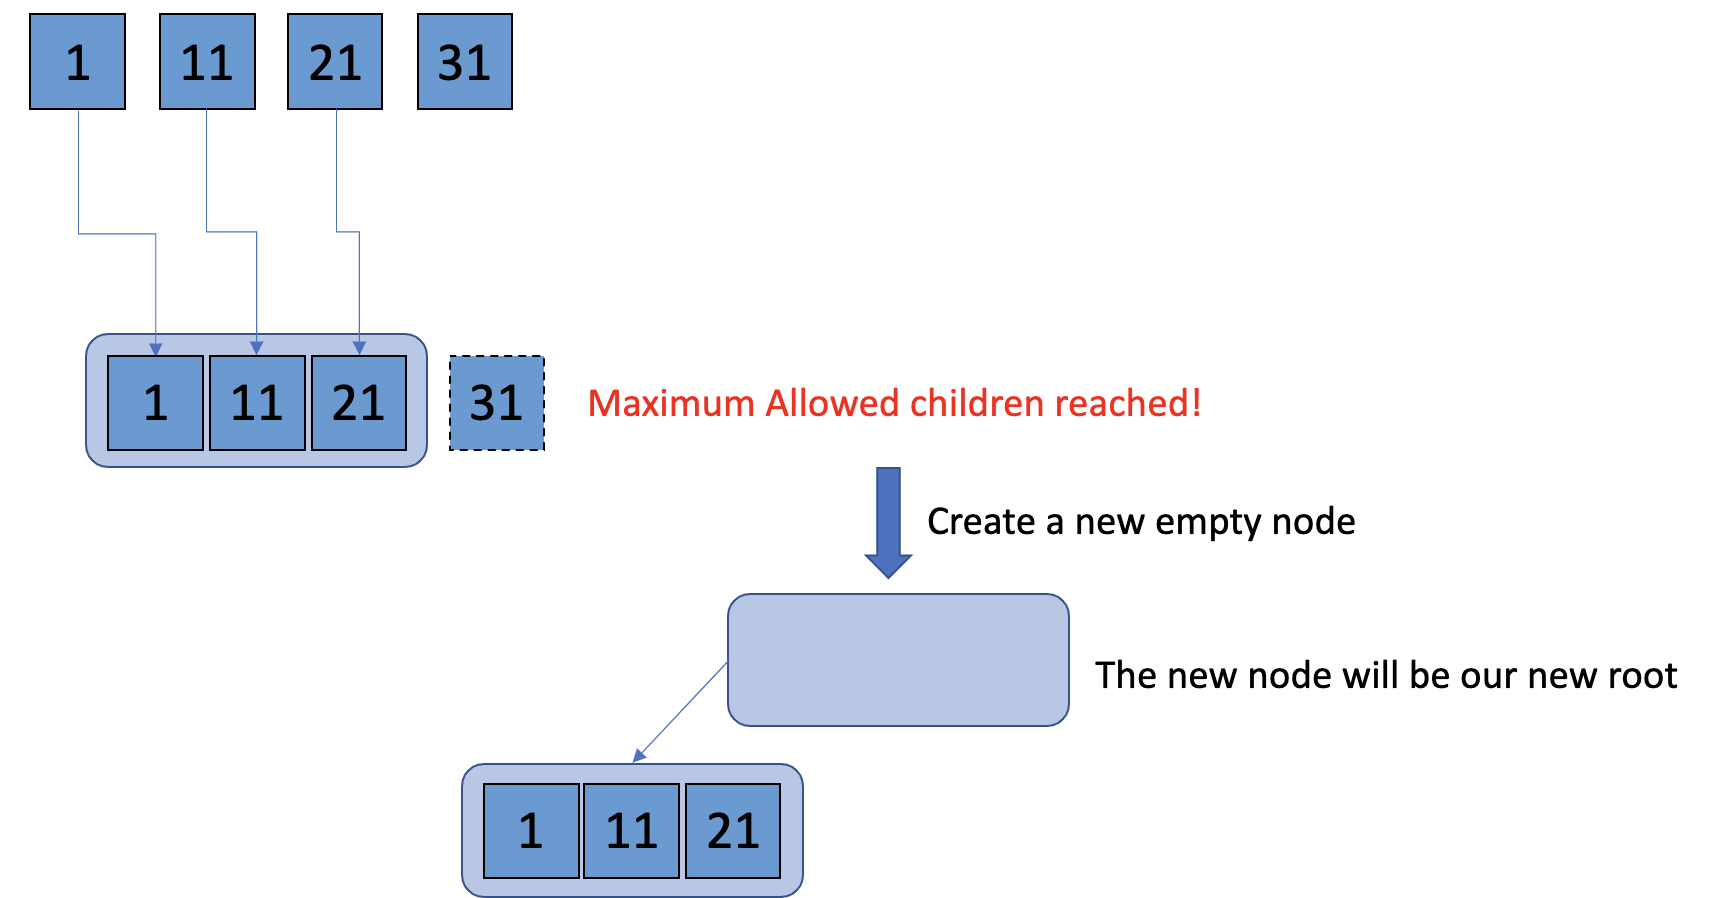
\includegraphics[width=0.6\textwidth]{graphs/B-Tree_example01.png}
    \caption{B-Tree key insertion}
    \label{fig:B-Tree key insertion1}
\end{figure}

\begin{figure}[htp]
    \centering
    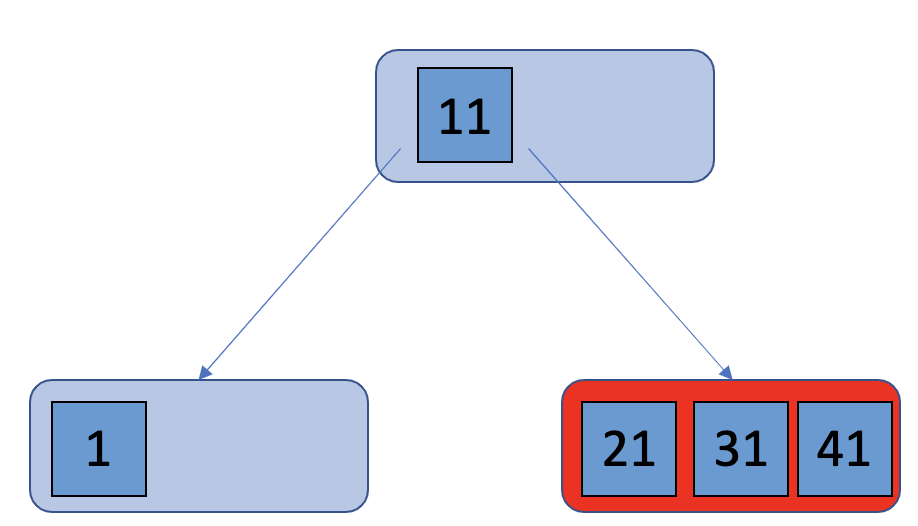
\includegraphics[width=0.3\textwidth]{graphs/B-Tree_example02.png}
    \caption{B-Tree key insertion}
    \label{fig:B-Tree key insertion2}
\end{figure}

\subsubsection{Insertion in a B-Tree}

\begin{algorithm}[H]
    \SetAlgoLined
    \SetKwInOut{Input}{Input}
     \Input{\texttt{$m$:order\_of\_tree ,$(k,v)$:(key, value), $N$:Node;}}
    \SetKwInOut{Output}{Output}
     \Output{\texttt{B-Tree}}
     \eIf{$N$ is a leaf and not yet full}  
     {
        \texttt{insert $(k,v)$ into $N$}
     }
     {
        \texttt{create new Node N'}\\
        \texttt{Find the median of the node}\\
        \texttt{Add the value at the median location to the new node N'}\\
     }
    \If{$N$ is root with no children and not full}
    {
    
        \texttt{insert $(k,v)$ into $N$}
        
    }
     \caption{Algorithm for B-Tree insertion}
     \label{B-Tree Insertion}
\end{algorithm}

There are two conditions in insertion:

\begin{itemize}
\item
\textbf{When the node is empty or not created at all}:
In the algorithm, initially when the first key is inserted and there is no root to the tree it will check the condition if there are any nodes and if not create a new one. It will insert the new key in the node and keeps inserting the new keys until it is one less than the order of the B-Tree being created. 
\item
\textbf{When the node is full}:
As soon as the maximum number of allowed children has reached for the root node a new empty node is created. Suppose we have inserted [1,11,21] to a node of a B-Tree with degree 4. Now if we want to insert a new value 31 into the tree, since it has reached the maximum number of children it will find the median of the existing node [1,11,21] which is 11 and increase the level of the B-tree to 2 and make [1] and [21] child nodes of [11]. So now if a new value is to be inserted it can be inserted. Splitting of the node happens each time it reaches it's maximum allowed keys. Now 31 will be compared with 11 and since 31 > 11 it will be inserted in the right child and it will have an updated value of [21,31]. More keys can then be inserted until it reaches it's maximum and splits again. Once the node is split it's parent is also updated to the median value i.e., [11] in this case for nodes [1] and [21,31,41] as can be seen in \ref{fig:B-Tree key insertion2}.
\end{itemize}

\subsubsection{Search in a B-Tree}

\begin{algorithm}[H]
    \SetAlgoLined
    \SetKwInOut{Input}{Input}
     \Input{\texttt{k ; key, root ; Root of the B-Tree}}
    \SetKwInOut{Output}{Output}
     \Output{\texttt{Value associated with key}}
     \For{$i\gets0$ \KwTo $len(Root Node)$}{
         \If{keys in root greater than k}
         {
            \texttt{SEARCH\_CHILD(key)} //Search linearly the child associated with the key location one before\\
            \eIf{Child is a leaf}
            {
                \texttt{Linearly search until the key is reached}
            }
            {
                \texttt{SEARCH\_CHILD(key)}
            }
            
         }
    }
     \caption{Algorithm for B-Tree Search}
     \label{B-Tree Search}
\end{algorithm}

Search in a B-Tree is basically the comparison of the value of the key that needs to be searched with the keys in the node. It first linearly checks the value in the root key and looks for a key value which is greater than the searched key. As soon as it finds a key greater than the searched key it will search in the child of the key before it. For example if we were to search of key [41] in the example of the B-Tree used above, we would first check the value [11] and since it smaller than [31] and there are no keys greater than this in the root node it will search in the right child of the root node. It will then linearly search the node and locate it's associated value and return it. 